\subsection{One polarization (NLSE case)}

\begin{figure}[tbp]
    \centering
        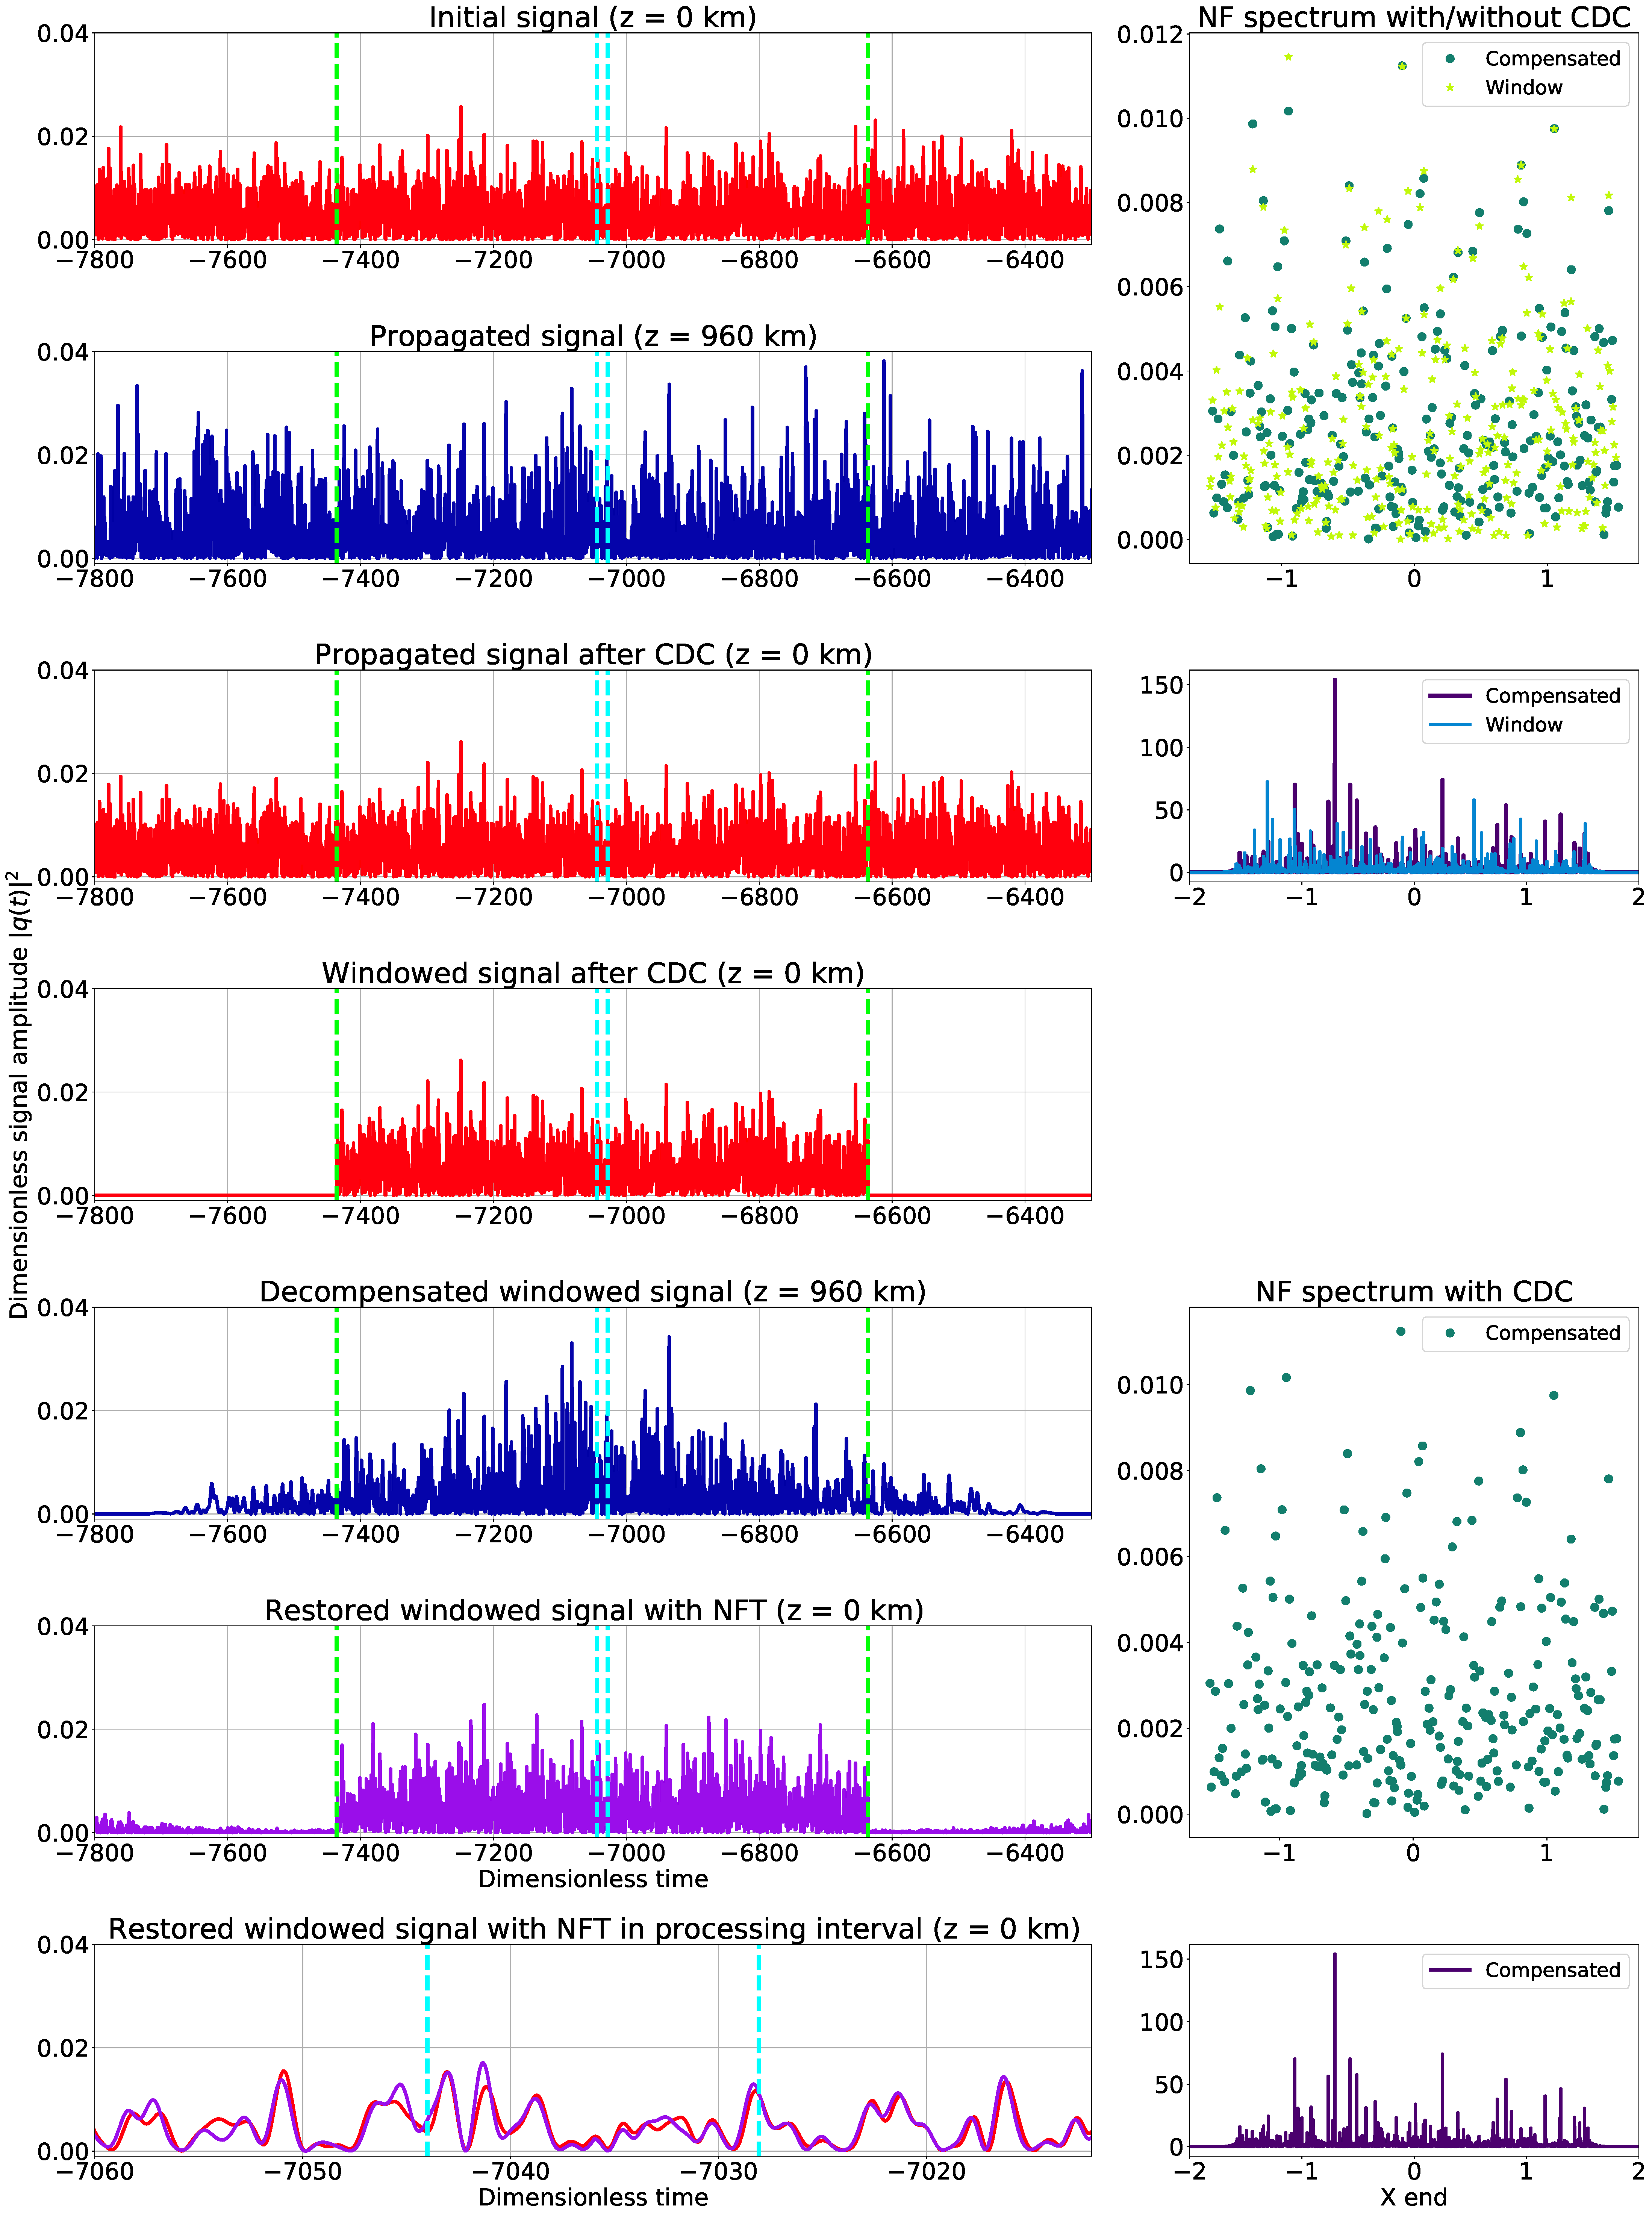
\includegraphics[width=0.95\linewidth]{images/window/nft_windowed_cdc_scheme.pdf}
    \caption{Scheme of using compensated window mode. The \textbf{left} column shows the signal processing steps. The \textbf{right} column shows an example of a signal NF spectrum processed without dispersion precompensation (window) and with the method described above (compensated).}
    \label{fig:nft_windowed_scheme}
\end{figure}

The first step in researching the window method was to apply it to the NLSE as a simpler model on which we could determine the method's areas of applicability. The application of the window method to the Manakov equations will impose additional restrictions due to the complexity of the model. Additionally, calculations for the NLSE are faster.

To evaluate the effectiveness of the proposed method, we utilized a single-channel 16-\acrshort{qam} \gls{wdm} signal~(see Eq~\eqref{eq:nlse_att}). 
Simulations involved transmitting the signal over $12 \times 80$ $[\textrm{km}]$ spans of standard single-mode fiber (SSFM), complemented with distributed Raman amplification (DRA). Two scenarios were considered: one noiseless scenario and another with DRA noise, mimicking an erbium-doped fiber amplifier noise figure of $4.5$ $[\textrm{dB}]$. The fiber had an attenuation coefficient of $\alpha = 0$ $[\textrm{dB}/\textrm{km}]$, a dispersion coefficient of $D = 16.8$ $[\textrm{ps}/\{\textrm{nm} \cdot \textrm{km}\}]$, and a nonlinear coefficient of $\gamma = 1.2$ $[\textrm{W} \cdot \textrm{km}]^{-1}$. Calculations were performed with 2 samples per symbol.

% In this study, we examined two scenarios: the first scenario involved analyzing the system without any EDFA noise, while the second scenario involved analyzing the system with EDFA noise characterized by a noise figure of $4.5$ $[\textrm{dB}]$. The simulations were conducted using a model of SSFM at a wavelength of $\lambda = 1550$ $[\textrm{nm}]$. The fiber was characterized by an attenuation coefficient of $\alpha = 0.2$ $[\textrm{dB}/\textrm{km}]$, a dispersion coefficient of $D = 16.8$ $\textrm{ps}/[\textrm{nm} \cdot \textrm{km}]$, and a nonlinear coefficient of $\gamma = 1.2$ $[\textrm{W} \cdot \textrm{km}]^{-1}$.

% Below is a table presenting BER values for signal reconstruction using NFT in window mode (NFT) and NFT in compensated window mode (NFT-CDC). The signal power level was $-4$ dBm. These results were obtained without additional signal equalization after NFT. The inclusion of additional filters may lead to improved results.

% \begin{table}[h!]
% \centering
% \begin{tabular}{|c|c|c|}
% \hline Distance, km & BER for NFT & BER for NFT-CDC \\
% \hline 560 & 0.0632 & 0.0273 \\
% \hline 640 & 0.0632 & 0.0264 \\
% \hline 720 & 0.0645 & 0.0156 \\
% \hline 800 & 0.0645 & 0.0117 \\
% \hline 880 & 0.0712 & 0.0273 \\
% \hline 960 & 0.0732 & 0.0234 \\
% \hline
% \end{tabular}
% \caption{BER values for signal reconstruction using NFT in window mode (NFT) and NFT in compensated window mode (NFT-CDC). Signal average power is $-4$ dBm.}
% \label{tab:ber_nft_cdc}
% \end{table}



Figure~\ref{fig:nft_windowed_scheme} illustrates the scheme for utilizing the compensated window mode. The left column displays the signal processing steps. The first plot depicts the initial continuous signal, while the second plot illustrates its propagation over a specified distance $z$. The third plot showcases the signal after dispersion compensation. Subsequently, the fourth graph demonstrates how the dispersion-compensated signal is windowed within a selected interval. This interval is carefully chosen to ensure that the central (processing) interval remains unaffected by the dispersion spreading from the cut portions of the signal. In the fifth step, dispersion is reintroduced to the signal. Finally, the sixth plot displays the result of NFT reconstruction of the initial signal. Consequently, the central interval of the signal is restored, denoted by the cyan vertical straight lines. After processing one interval, we proceed to the next, sequentially processing the entire signal.

The right column provides an example of an NF spectrum of a signal processed without dispersion precompensation (window) and with the method described above (compensated).
%
In the upper graph, which compares the two spectra, a notable feature in the discrete spectrum becomes apparent: when examining the maximum eigenvalues in the imaginary part, it becomes evident that some of them coincide. Conversely, another subset of the windowed-mode points deviates from the compensated-mode points (we are specifically considering only the maxima in the imaginary part). We attribute this deviation to the influence of the external (clipped) segments of the signal on the processed interval.

% We are currently studying the impact of point drift on the quality of signal reconstruction using NFT. We hypothesize that by effectively compensating for the error in discrete eigenvalues (particularly at points with the largest imaginary part, indicating the highest energy), we can substantially enhance the overall performance of NFT.

\begin{figure}[tbp]
    \centering
        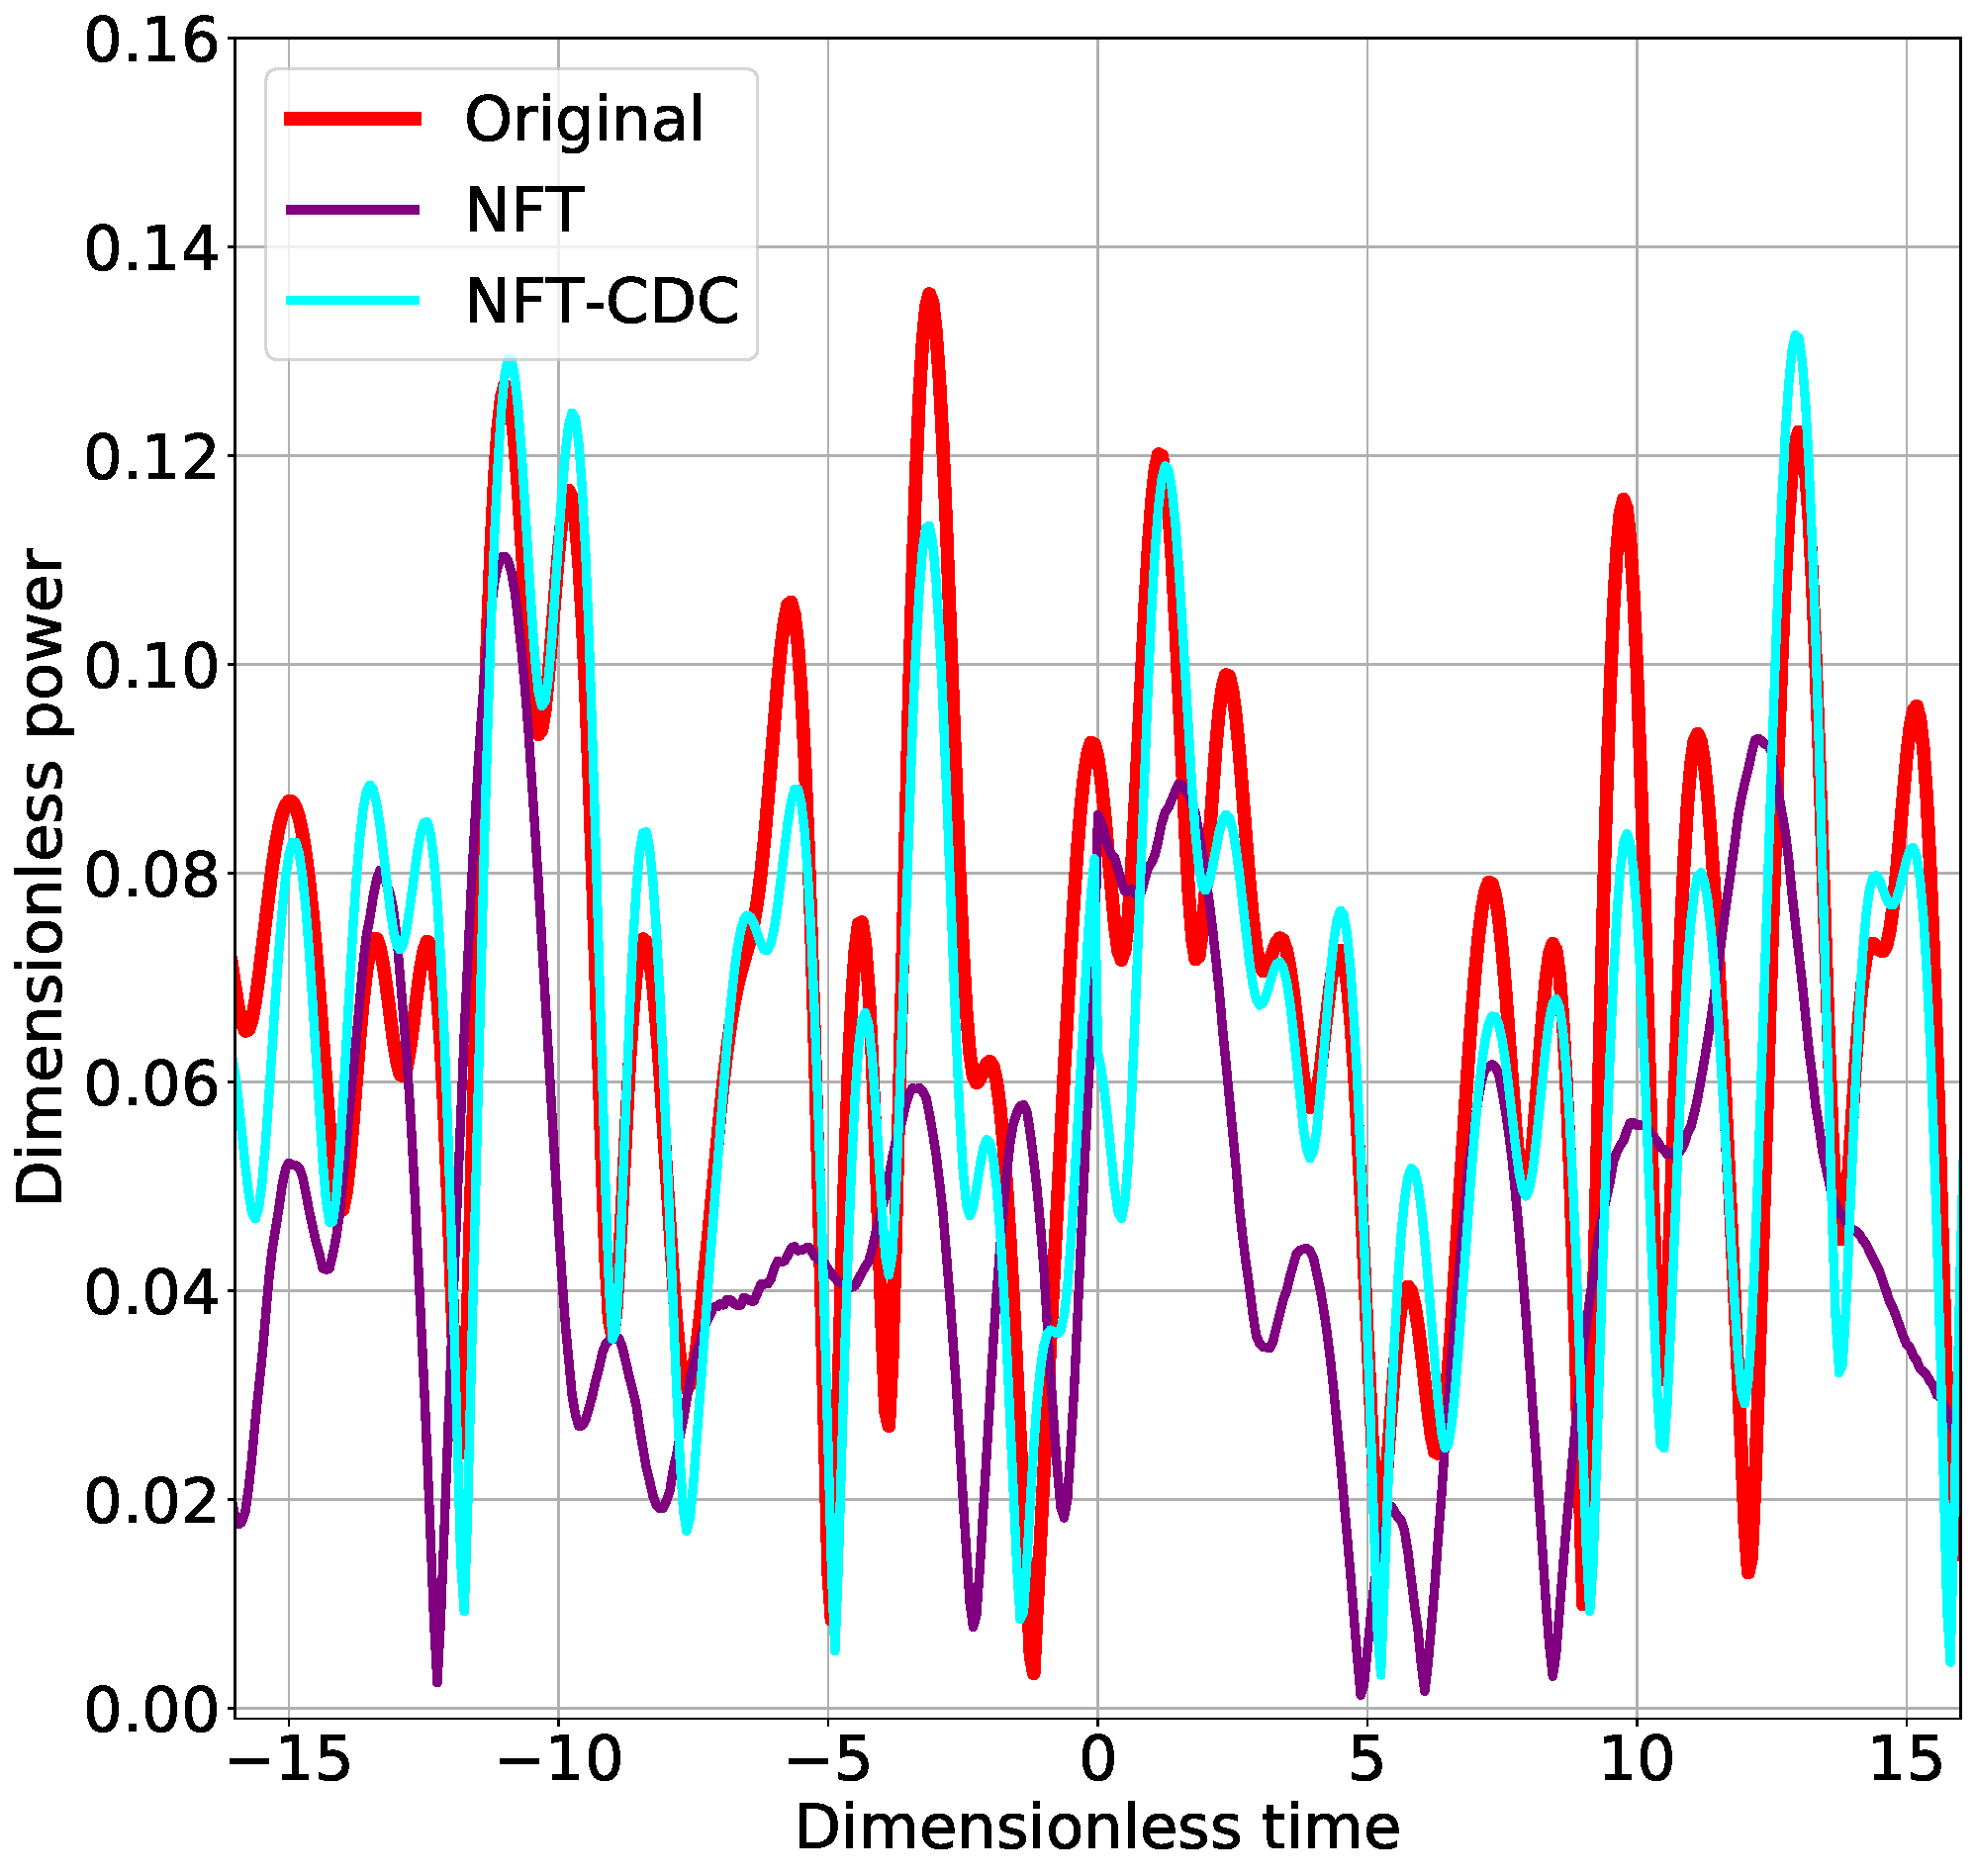
\includegraphics[width=0.5\linewidth]{images/window/nft_comp_cdc_m4dbm_final.pdf}
    \caption{Example how NFT algorithm restore initial signal (red). Cyan -- window mode with preprocessed chromatic dispersion compensation, purple -- NFT restoration for window mode.}
    \label{fig:nft_dbp_nft_and_cdc}
\end{figure}

In Fig.~\ref{fig:nft_dbp_nft_and_cdc} shows a comparison of the algorithms for NFT-CDC (dispersion precompensated) and for NFT without additional processing.
It can be seen from the graph that although the NFT tries to repeat the waveform, it lacks reconstruction accuracy. For a pre-compensated signal, the reconstruction accuracy is higher. We also noticed that, thanks to this approach, we automatically satisfy the condition of zeroing the boundary conditions at the ends of the time interval to use the forward NFT. Thus, there is no need to fictitiously select a function at the ends of the signals for zeroing. This also reduces the error received.



The presented approach has several parameters for optimization, such as $T_{proc}$, $R_D$, and the full window size $T_{w}$. For a corresponding propagation distance of 960 km, the dispersion length $T_d$ equals 297 symbols or approximately $440$ ps with $T_s=14.8$ ps.

We performed the inverse NFT using the fast layer-peeling method from the FNFT library (Ablovitz-Ladick scheme)~\cite{Wahls2016}. It operates only with a number of computational nodes equal to the degree of 2. Therefore, for such a long propagation distance, the minimum $T_w$ must be at least equal to 1024 ($\approx 1.5$ ns) to include $2 T_d$ intervals. We also considered a window size of 2048 symbols ($\approx 3$ ns) in total. The symbol interval of 4096 symbols turned out to be too large for numerical computations due to the $\mathcal{O}(N \log^2 N)$ complexity growth.

Direct NFT was performed in two separate steps. First, the phase jump tracking (PJT)~\cite{chekhovskoy2020introducing, 9542265} with an adaptive step size was applied for discrete eigenvalue search. This method used an effective exponential scheme of 6th order (ES6) with Pad\'e approximation of the matrix exponential~\cite{Medvedev2022}. Despite this, the discrete eigenvalue search was the most time-consuming step of one calculation.
%
Second, continuous spectrum computation was carried out using the fast FNFT\_TES4\_5B scheme~\cite{Medvedev2020_OE, Prins2018a}, which provided the most stable results in conjunction with the inverse FNFT scheme.
%
We used upsampling of the continuous spectrum by a factor of up to 16 times to enhance the stability of the inverse transform and improve the accuracy of phase jump detection on the real axis.

% \begin{figure}[pbt]
%     \centering
%     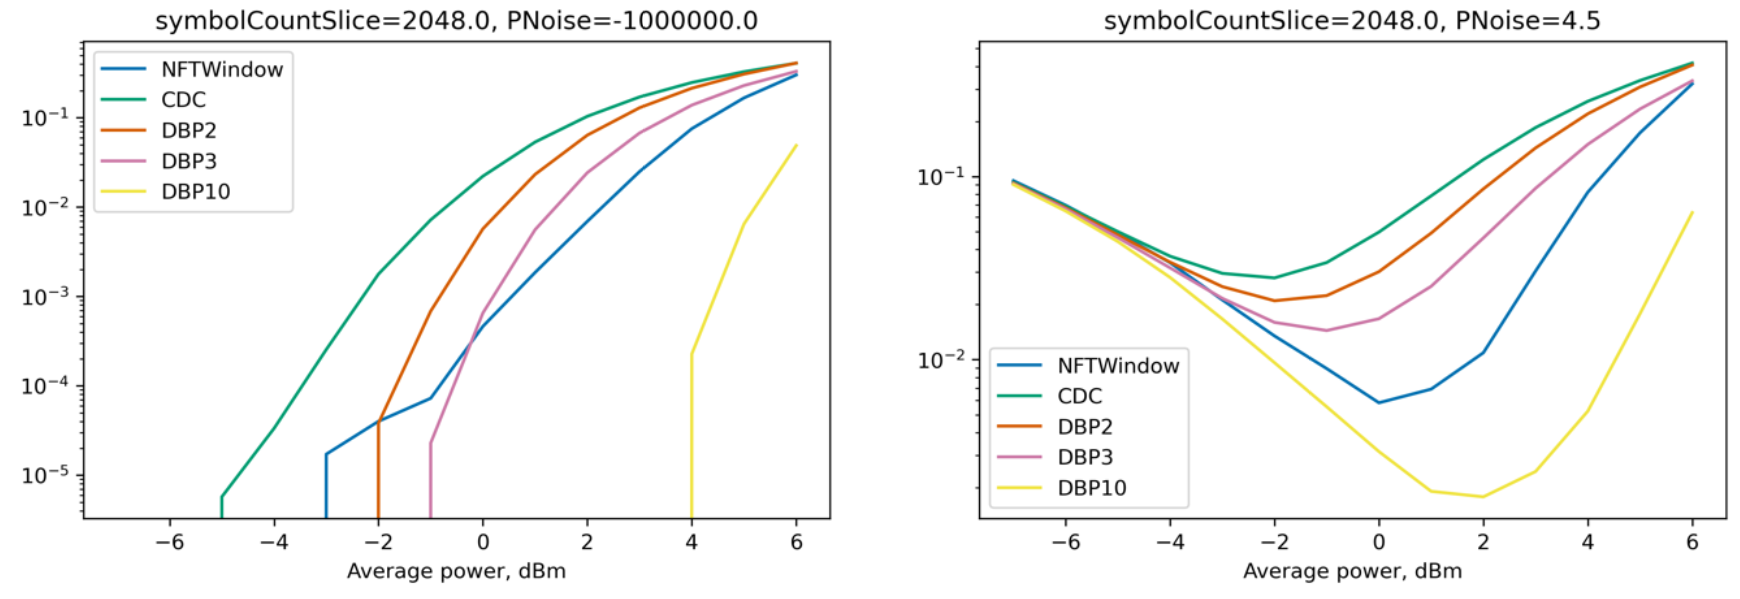
\includegraphics[width=1.0\linewidth]{images/window/ber_window.PNG}
%     \caption{The dependence of BER versus the average signal power $P_0$. The left column corresponds to the noiseless case, the right column corresponds to the noise power of $4.5$ dB. Total window size is $T_w=2048$. Processed symbol count $T_{proc} = 512$. The dispersion broadening scale factor $R_d=1.2$.}
%     \label{fig:noise_all}
% \end{figure}

\begin{figure}[tpb]
    \begin{minipage}[h]{0.5\linewidth}
    \center{
        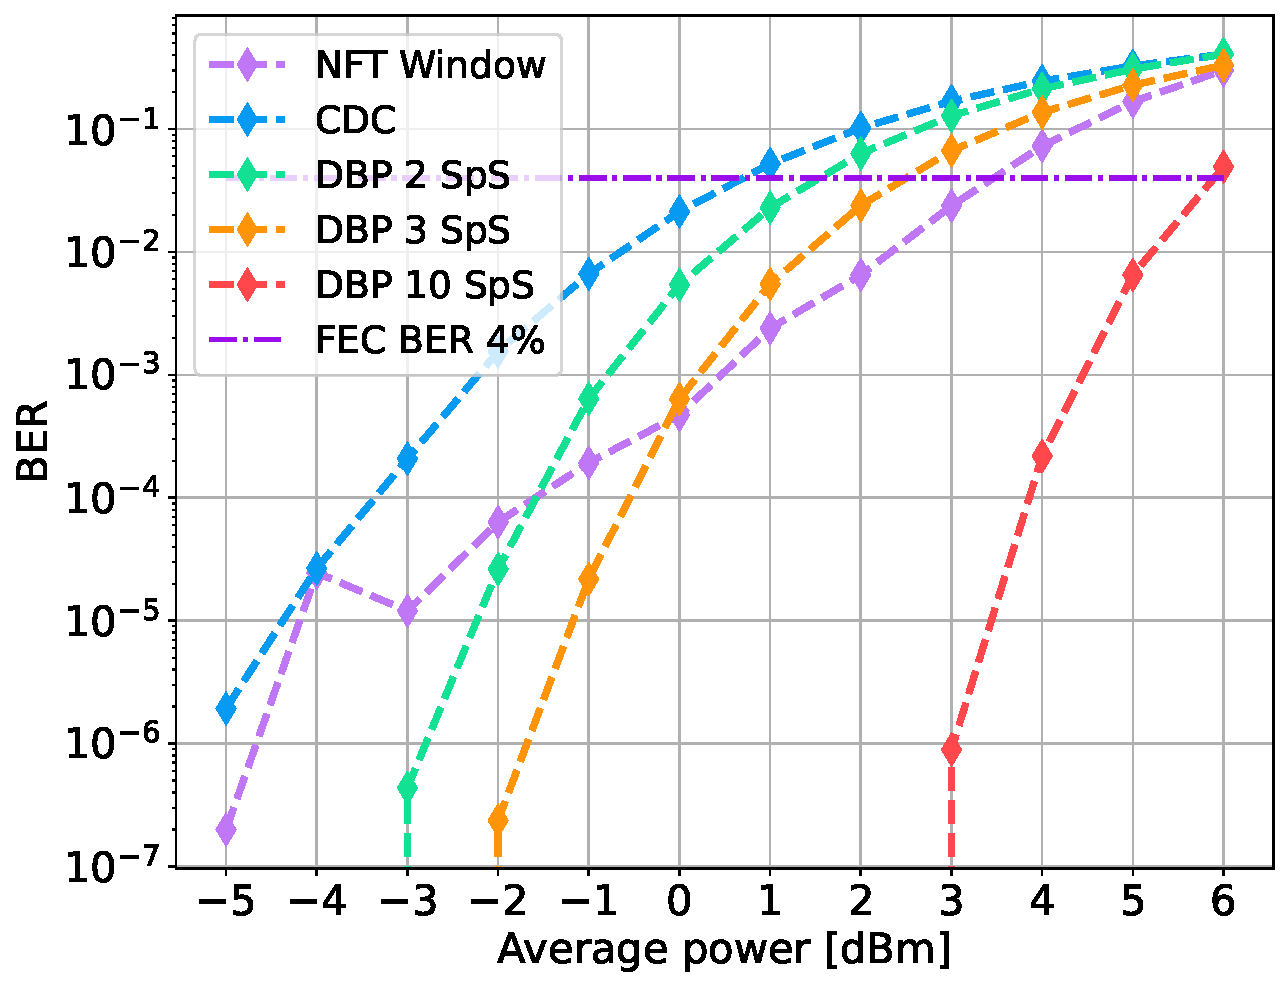
\includegraphics[width=1\linewidth]{images/window/ber_nft_window_wo_noise.pdf}
    }
    \end{minipage}
    \hfill
    \begin{minipage}[h]{0.5\linewidth}
    \center{
        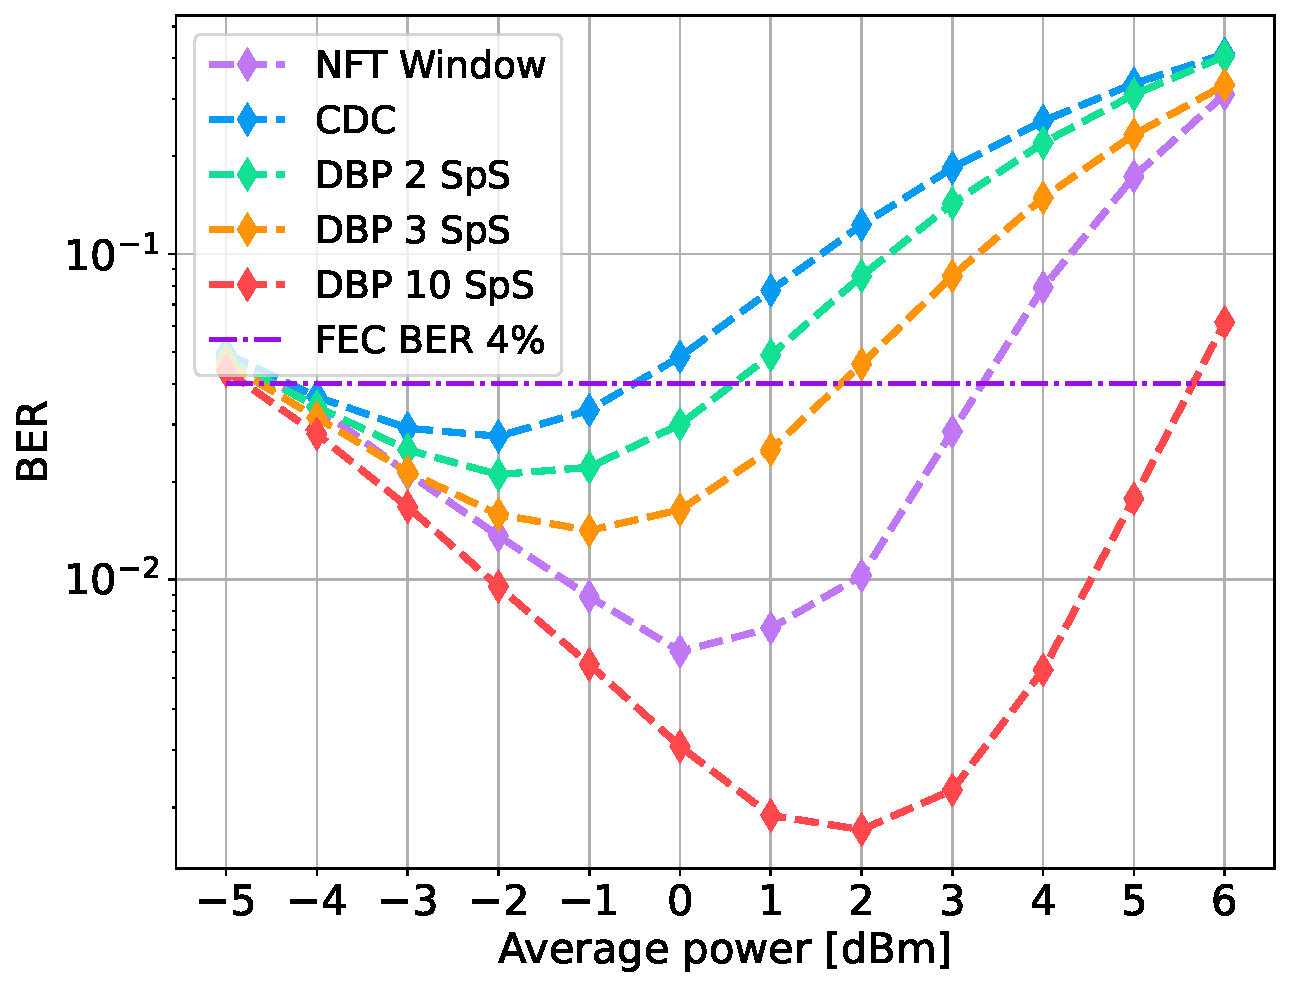
\includegraphics[width=1\linewidth]{images/window/ber_nft_window.pdf}
    }
    \end{minipage}
    \vfill
    \begin{minipage}[h]{0.5\linewidth}
    \center{
        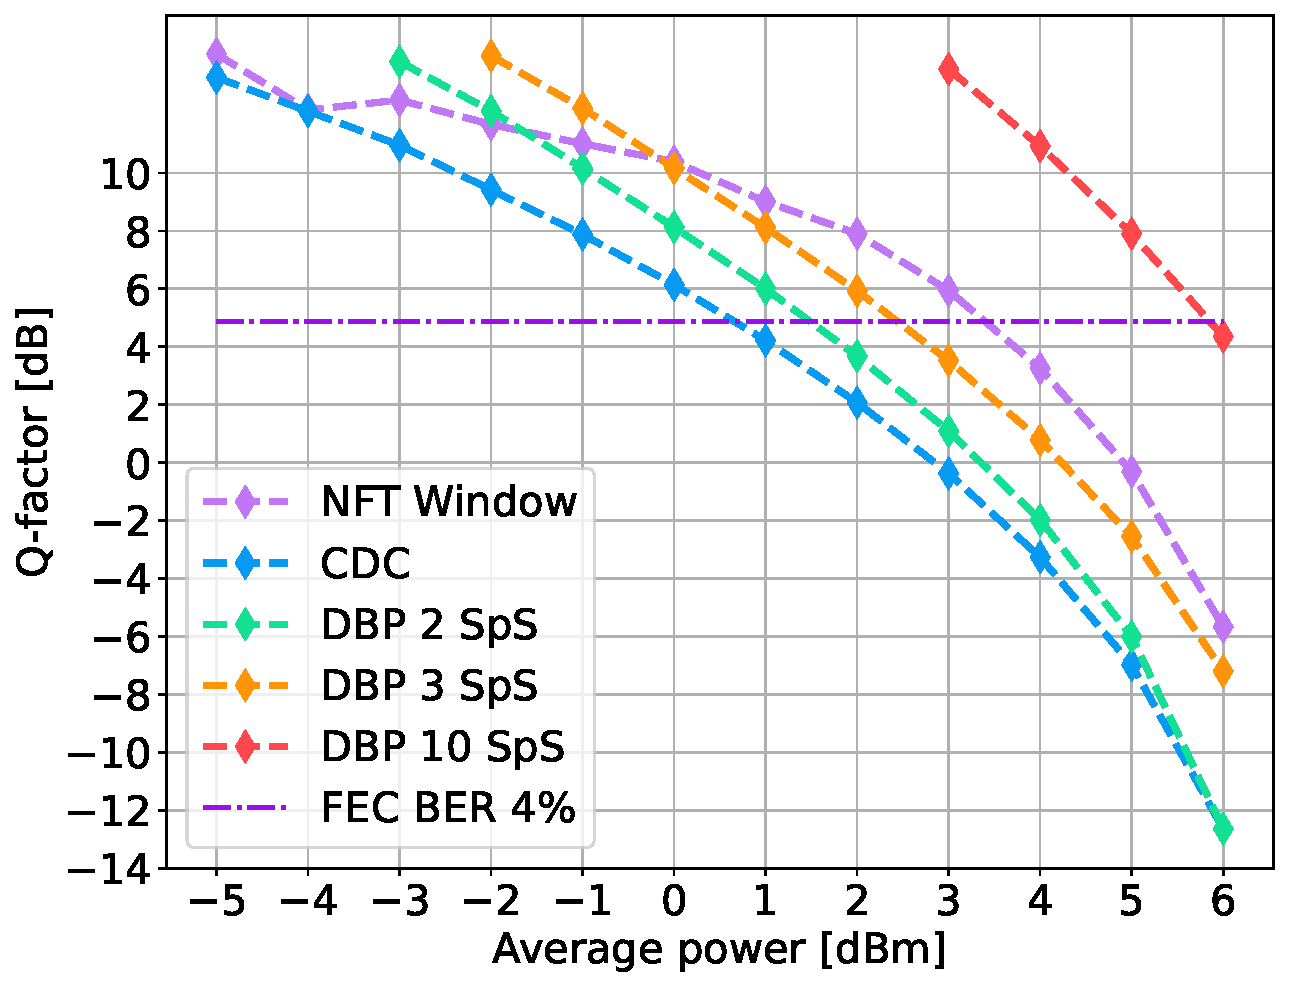
\includegraphics[width=1\linewidth]{images/window/q_nft_window_wo_noise.pdf}
    }
    \end{minipage}
    \hfill
    \begin{minipage}[h]{0.5\linewidth}
    \center{
        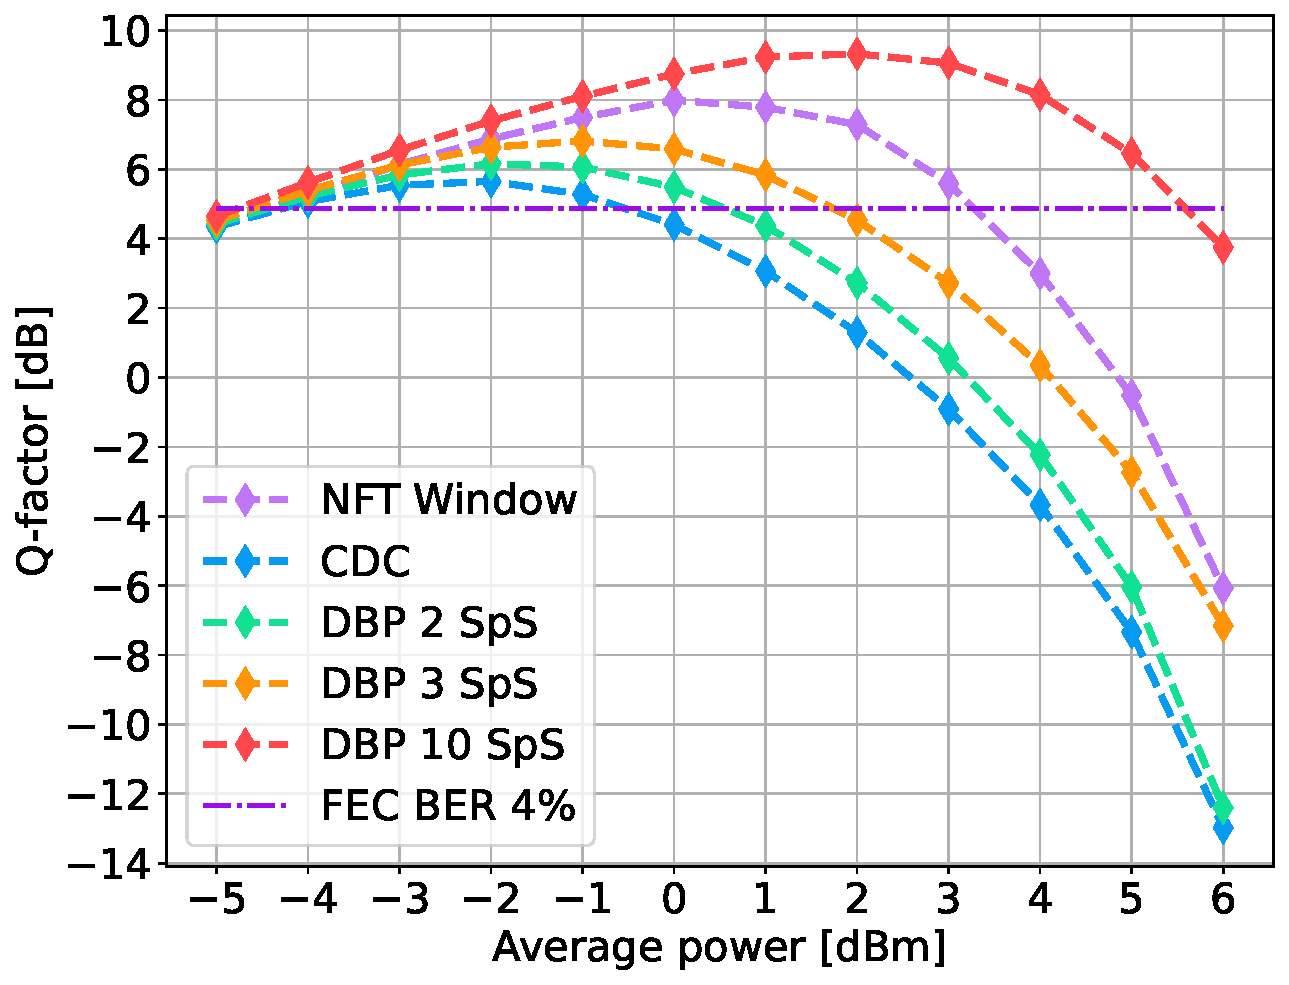
\includegraphics[width=1\linewidth]{images/window/q_nft_window.pdf}
    }
    \end{minipage}
    \caption{The dependence of BER (upper row) and Q-factor (lower row) versus the average signal power $P_0$. The \textbf{left column} corresponds to the noiseless case, the \textbf{right column} corresponds to the noise power of $4.5$ dB. Total window size is $T_w=2048$. Processed symbol count $T_{proc} = 512$. The dispersion broadening scale factor $R_d=1.2$.}
    \label{fig:noise_all}
\end{figure}

One of the key practical considerations in our study is determining the appropriate processing interval size, $T_{proc}$. To minimize additional computational effort compared to the conventional approach, we aimed to maximize the processing interval size. Our investigations revealed that a window of $T_w=2048$ symbols is a more promising approach, as its wide zero tails ($T_z$) result in a small step in the frequency domain, which improves the accuracy of optical field restoration.

In our subsequent investigations, we adopted a dispersion broadening scale factor of $R_d=1.2$, when processed symbol count was set to $T_{proc} = 512$. We also examined the influence of noise on different values of the average power $P_0$. Figure~\ref{fig:noise_all} presents a comparison between the noiseless case and the case with noise of power 4.5 dBm. We found that the presence of noise only slightly increases the discrete spectrum size.

Across all considered average power values, the NFT window approach outperformed DBP with 2 steps per span in terms of bit error rate (BER) and error vector magnitude (EVM). In some nonlinear regimes, the NFT approach demonstrated a greater accuracy than DBP with 3 steps per span. However, it should be noted that the accuracy of the NFT approach cannot be compared to that of DBP with 10 steps per span.


\subsection{Two polarization (\acrshort{me} case)}

The dual-polarization scheme introduces a second polarization for the NLSE equation and the interactions between the two polarizations. For real-world parameters, the effects of the presence of two polarizations are sufficiently small and can be neglected in the first-order approximation. Therefore, we use the approach, introduced in the paper~\cite{Civelli2019}, to deal with DP signals.
The authors introduced a novel dual-polarization transmission scheme with reduced complexity that separately processes each polarization component. Instead of applying the more complex $\text{NFT}_\text{M}$ -- the NFT approach based on the Manakov equation for encoding and decoding information on the nonlinear spectrum -- they proposed using independent $\text{NFT}_\text{NLS}$ processing based on the NLSE channel for each polarization component of the signal. They demonstrated that, in a certain range of system parameters where performance is dominated by the effect of noise on the nonlinear spectrum, such reduced complexity processing can even provide a performance improvement compared to full vector processing, despite the mismatch between the channel model and processing.

Thus, we processed each polarization separately using NFT for NLSE. This approach proved to be effective, and we managed to achieve a high level of performance.

% \begin{figure}[!hbt]
%     \centering
%     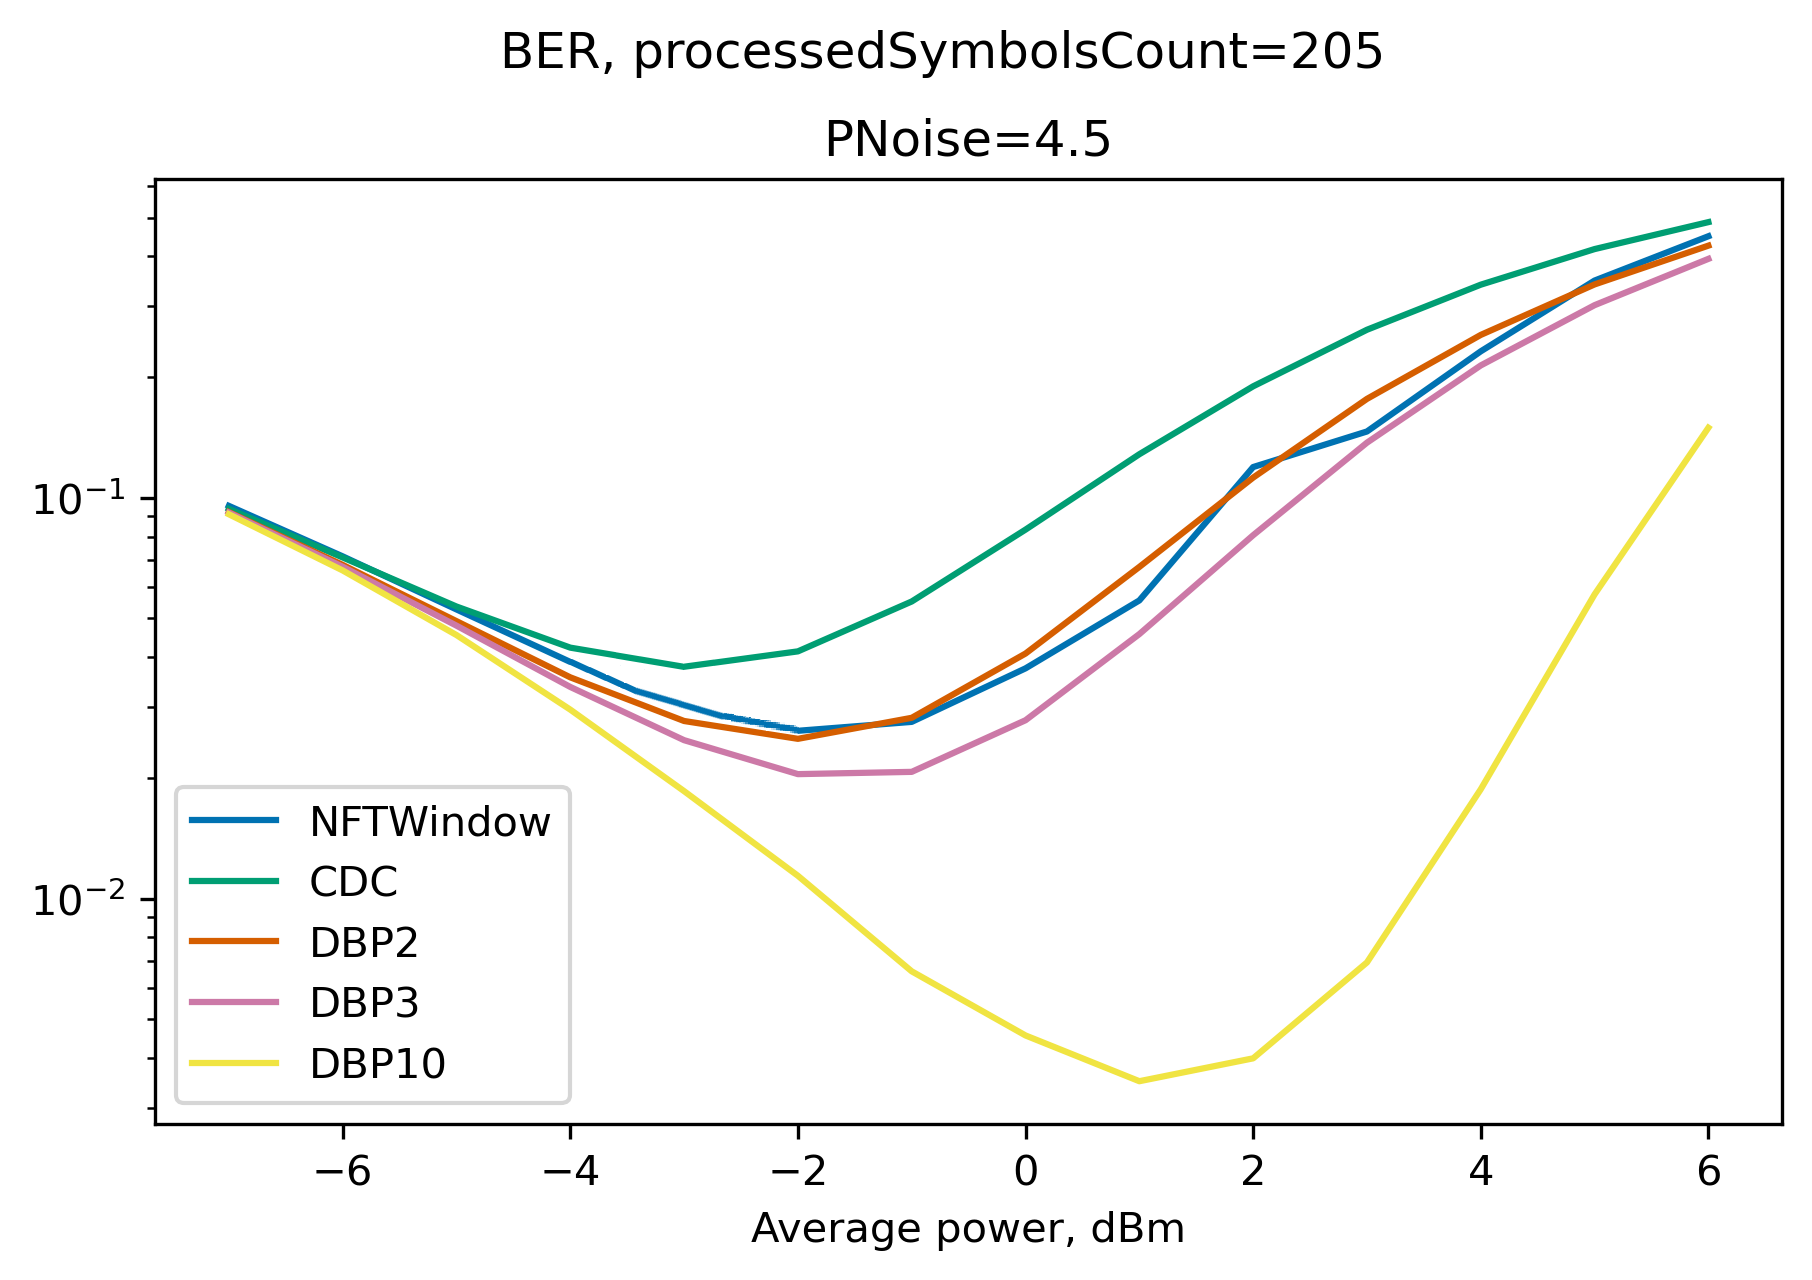
\includegraphics[width=0.6\linewidth]{images/window/BER_processedSymbolsCount=205.png}
%     \caption{The dependence of BER versus the average signal power $P_0$. The left column corresponds to the noiseless case, the right column corresponds to the noise power of $4.5$ dBm. Total window size is $T_w=2048$. Processed symbol count $T_{proc} = 512$. The dispersion broadening scale factor $R_d=1.2$.}
%     \label{fig:noise_ME}
% \end{figure}

\begin{figure}[tpb]
    \begin{minipage}[h]{0.5\linewidth}
    \center{
        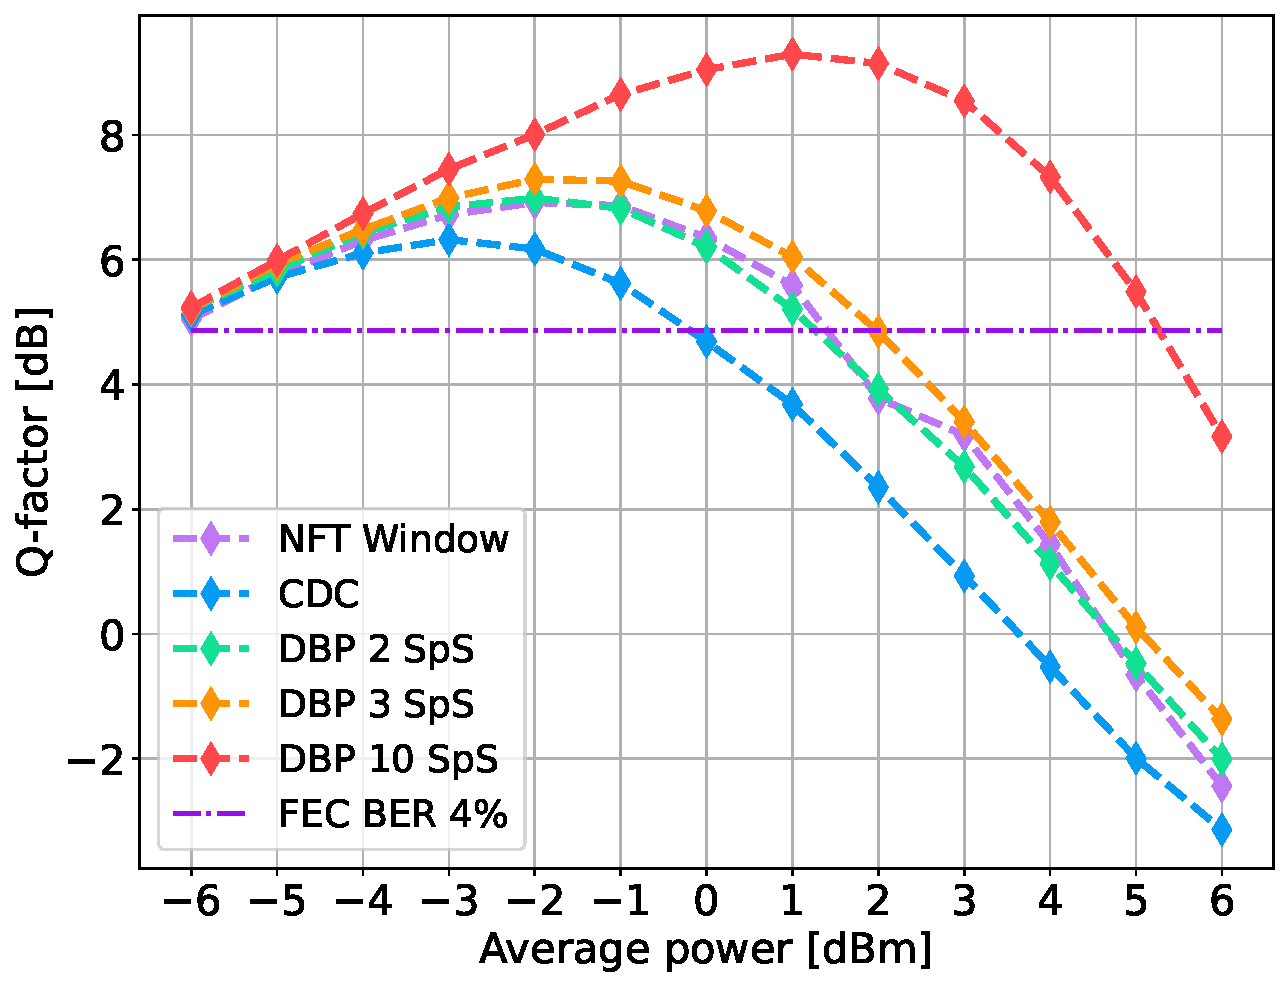
\includegraphics[width=1\linewidth]{images/window/q_nft_manakov_window.pdf}
    }
    \end{minipage}
    \hfill
    \begin{minipage}[h]{0.5\linewidth}
    \center{
        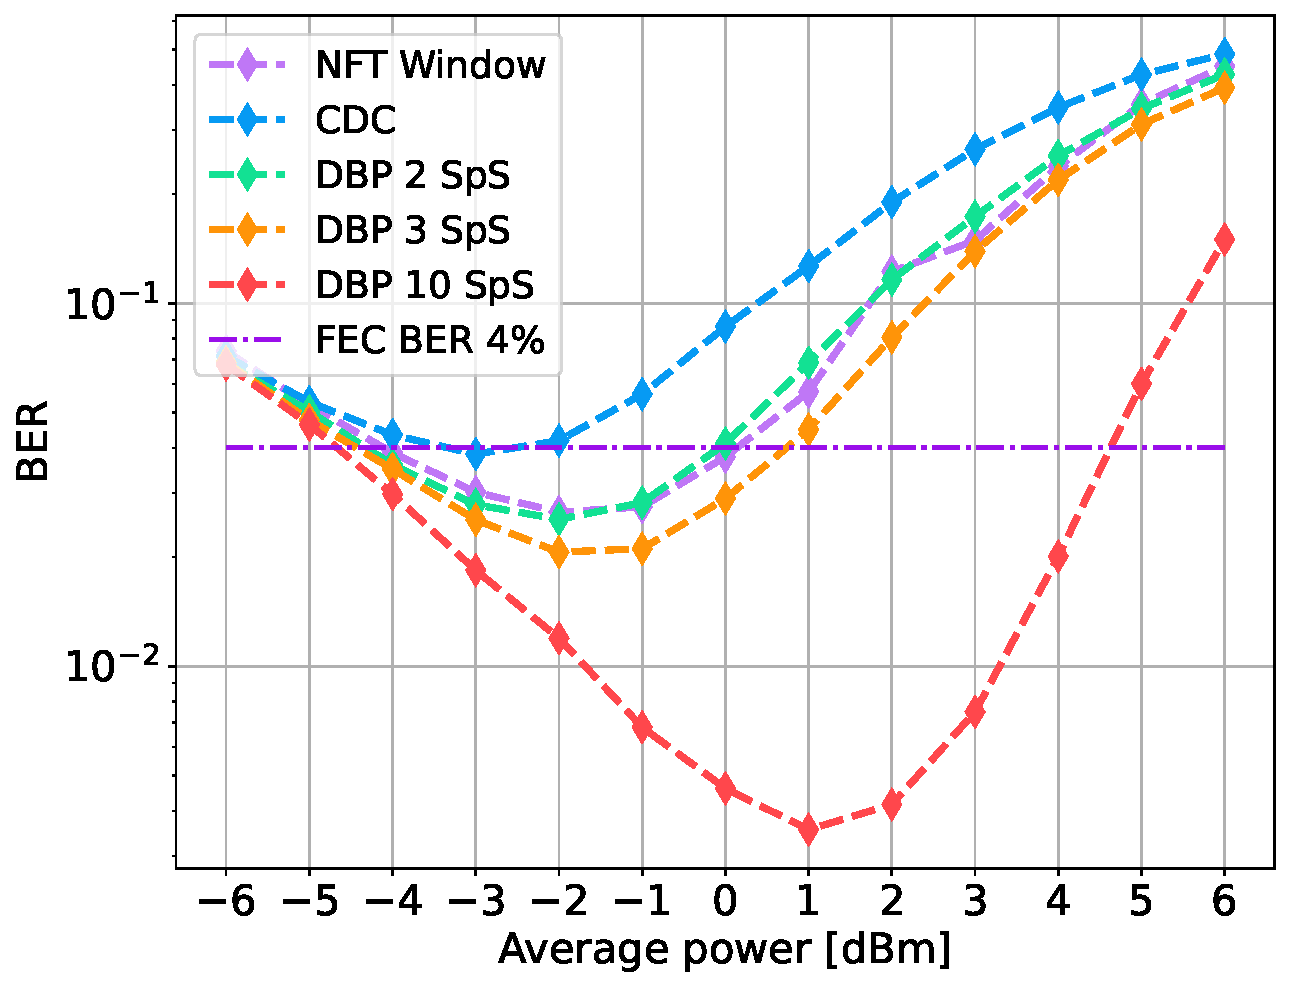
\includegraphics[width=1\linewidth]{images/window/ber_nft_manakov_window.pdf}
    }
    \end{minipage}
    \caption{The dependence of BER \textbf{(left)} and Q-factor \textbf{(right)} versus the average signal power $P_0$. The left column corresponds to the noiseless case, the right column corresponds to the noise power of $4.5$ dBm. Total window size is $T_w=2048$. Processed symbol count $T_{proc} = 512$. The dispersion broadening scale factor $R_d=1.2$.}
    \label{fig:noise_ME}
\end{figure}

One projection of BER values for 12 spans is presented in Fig.~\ref{fig:noise_ME}. Here, the result was obtained by averaging over 100 launches for each value of the average power $P_0$. When compared to signal recovery, which was modeled by NLSE, accuracy degradation is noticeable. Previously, NFT allowed signal recovery with higher accuracy than that of DBP with 3 steps per span. Now, NFT is applied separately to each polarization. However, the accuracy of a 2-step/span DBP is achieved, and for higher powers, the accuracy approaches that of a 3-step/span DBP.


